%%%%%%%%%%%%%%%%%%%%%%% file template.tex %%%%%%%%%%%%%%%%%%%%%%%%%
%
% This is a general template file for the LaTeX package SVJour3
% for Springer journals.          Springer Heidelberg 2010/09/16
%
% Copy it to a new file with a new name and use it as the basis
% for your article. Delete % signs as needed.
%
% This template includes a few options for different layouts and
% content for various journals. Please consult a previous issue of
% your journal as needed.
%
%%%%%%%%%%%%%%%%%%%%%%%%%%%%%%%%%%%%%%%%%%%%%%%%%%%%%%%%%%%%%%%%%%%
%
% First comes an example EPS file -- just ignore it and
% proceed on the \documentclass line
% your LaTeX will extract the file if required
\begin{filecontents*}{example.eps}
%!PS-Adobe-3.0 EPSF-3.0
%%BoundingBox: 19 19 221 221
%%CreationDate: Mon Sep 29 1997
%%Creator: programmed by hand (JK)
%%EndComments
gsave
newpath
  20 20 moveto
  20 220 lineto
  220 220 lineto
  220 20 lineto
closepath
2 setlinewidth
gsave
  .4 setgray fill
grestore
stroke
grestore
\end{filecontents*}
%
\RequirePackage{fix-cm}
%
%\documentclass{svjour3}                     % onecolumn (standard format)
%\documentclass[smallcondensed]{svjour3}     % onecolumn (ditto)
\documentclass[smallextended]{svjour3}       % onecolumn (second format)
%\documentclass[twocolumn]{svjour3}          % twocolumn
%
\smartqed  % flush right qed marks, e.g. at end of proof
%
\usepackage[brazilian]{babel}
\usepackage[utf8]{inputenc}
\usepackage[T1]{fontenc}
\usepackage{natbib}
\usepackage{graphicx}

%
%\usepackage{mathptmx}      % use Times fonts if available on your TeX system
%
% insert here the call for the packages your document requires
%\usepackage{latexsym}
% etc.
%
% please place your own definitions here and don't use \def but
% \newcommand{}{}
%
% Insert the name of "your journal" with
 \journalname{Biodiversity and Conservation}
%
\begin{document}

\title{Distribution of rupicolous species endemic from Brazil in inselbergues  of the Atlantic Forest %\thanks{Grants or other notes
%about the article that should go on the front page should be
%placed here. General acknowledgments should be placed at the end of the article.}
}
%\subtitle{Do you have a subtitle? \\ If so, write it here}

\titlerunning{Brazilian species in inselbergues from the Atlantic Forest}        % if too long for running head

\author{
        Diogo S. B. Rocha  \and
        Beatriz Parreira da Cunha  \and
        Marinez F. de Siqueira  \and
        Rafaela Campostrini Forzza
}

%\authorrunning{Short form of author list} % if too long for running head

\institute{
           Diogo S. B. Rocha \at
           Jardim Botânico do Rio de Janeiro \\
           Pacheco Leão 915, 22460-030, Rio de Janeiro \\
           \email{diogosbr@gmail.com}
           \and
            Beatriz Parreira da Cunha \at
            PUC \\
            \email{beapcunha1@gmail.com}
            \and
           Marinez F. de Siqueira \at
           Jardim Botânico do Rio de Janeiro \\
           Pacheco Leão 915, 22460-030, Rio de Janeiro \\
           \email{marinez.siqueira1@gmail.com}
           \and
           Rafaela Campostrini Forzza \at
           Jardim Botânico do Rio de Janeiro \\ 
           Pacheco Leão 915, 22460-030, Rio de Janeiro \\
           \email{rafaela@jbrj.gov.br}
}

\date{Received: date / Accepted: date}
% The correct dates will be entered by the editor


\maketitle

\begin{abstract}
Insert your abstract here. Include keywords, PACS and mathematical
subject classification numbers as needed. 150 to 250 words
\keywords{inselbergs \and ecological niche model \and distribution patterns \and (4 to 6 keywords)}
% \subclass{MSC code1 \and MSC code2 \and more}
\end{abstract}

\section{Introduction}
\label{intro}
like\textsubscript{this}
Inselbergs are rocky outcrops that correspond to Precambrian Mountains, usually monolithic granite / gneiss \citep{bremer2000InselbergsGeomorphologyGeoecology}. They are distributed across various regions of the planet, but are most frequent in the landscape of southeastern Brazil, Madagascar and southwest Australia, and these three regions are identified as the hotspots of inselberg plants in the world \citep{porembski2007TropicalInselbergsHabitat}. The formation of these outcrops must have started around 20-2.6 Ma and, more recently, tectonic movements may have contributed to their final shape \citep{varajao2015PancasKingdomBornhardts}. They can occur as isolated hills on the plain or forming chains with individual outcrops situated at distances of only a few kilometers. These lowland monoliths are also known as “sugar loaf” \citep{porembski2000IslandsIslandsHabitatsa} and represent true “terrestrial islands,” similar to oceanic islands, having significant relevance as models for studies of evolutionary and ecological processes \citep{porembski2000IslandsIslandsHabitatsa}. 

In Brazil, inselbergues are found mainly in the Brazilian Caatinga biome, in the semiarid semiarid region, to the cold mountains of Rio Grande do Sul state \citep{safford2000SoutheastBrazil}. \cite{absaber1967DominiosMorfoclimaticosProvincias}, indicated the existence of six morphoclimatic domains in Brazil and considered sugar loaves in the “seas of hills” domain. Despite this large area of occurrence, it is in the Atlantic Forest domain that there is a region where they are found in great abundance and are considered important landscape component \citep{porembski2007TropicalInselbergsHabitat}. This region was recently named by \cite{depaula2016SugarLoafLand} as Sugar Loaf Land.

Inselbergues present extremely severe environmental conditions such as high temperature, high insolation, high evapotranspiration rate and restricted soil occurrence, which, in turn, leads to rapid water loss through runoff, being considered microclimatic deserts \citep{luttge2007PhysiologicalEcologyTropical, porembski2007TropicalInselbergsHabitat}. Although they have a relatively limited structure and extreme conditions, they cover a wide range of plant life and species richness \citep{porembski1998DiversityEcologySaxicolous, barthlott2000WhyStudyInselbergs, porembski2000InvasibilityTropicalGranite, bremer2000InselbergsGeomorphologyGeoecology}. Another interesting aspect is that the plant populations occurring in these outcrops generally exhibit spatial isolation and restricted gene flow \citep{barbara2008WithinpopulationSpatialGenetic, boisselier-dubayle2010GeneticStructureXerophilous, hmeljevski2017PlantPopulationsDistinct}. Due to these characteristics, the vegetation of these environments differs markedly from their surroundings, thus having a highly specialized flora and a large number of endemic species \citep{porembski1998DiversityEcologySaxicolous, porembski2007TropicalInselbergsHabitat}.

Floristic and ecological studies on inselbergues, though they are better known in the southeastern Brazilian landscape, are still few. However, we can mention here studies that have been carried out in the last two decades, contributing to an advance in the knowledge about the flora of Brazilian inselbergues, e.g.\citep{meirelles1999VegetationGraniteRock, parmentier2009ImpactEcologicalDifferentiation,porembski2007TropicalInselbergsHabitat, santos2010EstruturaVegetacaoArbustivoherbacea, depaula2016SugarLoafLand, paula2017FloristicEcologicalCharacterization}. These studies indicate a high number of endemic taxa, however, the low number of samples deposited in herbariums makes it difficult to understand their geographic distribution patterns \citep{depaula2016SugarLoafLand}.

The high degree of endemism, the isolation of populations and the ecological uniqueness of species occurring in inselbergs (e.g. low recruitment) make them excellent models for studies. In addition, habitat loss and fragmentation, degradation of inselbergs for ornamental rock extraction, the presence of invasive grasses that increase the occurrence of fires, and climate change are just examples of environmental changes caused by anthropogenic factors, with consequences on species distribution \citep{szarzynski2000XericIslandsEnvironmental, safford2000SoutheastBrazil, porembski2007TropicalInselbergsHabitat}. These growing threats require new technologies and analytical tools so that we can gain or deepen existing knowledge, assist in conserving groups of living things and landscapes \citep{peterson2002FutureProjectionsMexican, ortega-huerta2004ModellingSpatialPatterns}.
 
Ecological niche modeling (ENM) has become a common procedure for determining the extent of geographic distribution of species based on environmental characteristics. Computer modeling techniques can assist in the task of identifying areas at high risk of biodiversity loss, planning for the use of uninhabited regions, estimates of invasion risk, reintroduction and planning for threatened species protection \citep{guisan2005PredictingSpeciesDistribution, correa2011ComputationalTechniquesBiologic}. The theoretical basis of the ENMs is based on the concepts of fundamental niche (inferred through abiotic variables), but characterized by the potential niche (fundamental niche available in nature), inferred by the realized niche (influence of biotic interactions on potential niche) and effectively occupied, considering the movement capacity of species and their historical restrictions on dispersal \citep{colwell2009HutchinsonDualityOnce, soberon2009NichesDistributionalAreas}.

In practice, ENM processes simulate the spatial distribution of species by relating the distribution of species occurrence points in known locations to a multivariate set of environmental information, applying mathematical functions to generate geographically designed spatial predictions \citep{guisan2000PredictiveHabitatDistribution, guisan2005PredictingSpeciesDistribution}. \textit{For the formation of the model, the mathematical functions are applied by the algorithms, which are used to establish the nonrandom relationship between occurrence records and environmental variables}. The choice of algorithm is associated with several data characteristics, including: the type of environmental variable and the availability of absence and presence data, and the quantity and quality of available data  \citep{phillips2006MaximumEntropyModeling, peterson2011EcologicalNichesGeographic}. 

%OBJETIVOS

The objective of this study was to identify the biogeographic patterns of Inselbergues typical species (i.e. \textit{Encholirium horridum} L.B.Sm., \textit{Pilosocereus brasiliensis} (Britton & Rose) Backed., \textit{Pseudolaelia vellozicola} (Hoehne) Porto & Brade and \textit{Vellozia plicata} Mart.), answering the following questions: i) the species studied present similar niches? ii) endemic species of inselbergues have similar distribution patterns? iii) Which climatic variables most influence the species studied distribution? 

%\textbf{Como na descrição das espécies nós incluimos algumas coisas de polinização/dispersão de cada uma, eu pensei que poderíamos ter alguma pergunta tipo se os diferentes padrões teriam influência no padrão de distribuição das espécie. Vc acha possível?}

%
In the present paper, we aimed to generate new insights into regional-scale environmental drivers of geographic distributions of termite species, and how these environmental factors impact co-occurrence among congeneric species. Focusing on the southern Appalachian Mountains and surrounding areas, we performed an ENM-based evaluation of niche divergence among the three most common Reticulitermes species in the eastern United States. In addition to identifying niche divergence, if present, we aimed to determine the environmental factors driving niche divergence among species.
%


\section{Material and methods}
\label{mat_met}

\subsection{Species studied}

\textit{Encholirium horridum} L.B.Sm. (Figure \ref{encholirium}) forms large populations in inselbergues distributed mainly in the Espírito Santo state, with the limits of its geographic distribution being the south of Bahia state, east of Minas Gerais and north of Rio de Janeiro state \citep{hmeljevski2017PlantPopulationsDistinct}. It is an herbaceous, rupicolous species. Its main pollinators are bats and hummingbirds. The seed morphology indicates anemocoric dispersion, but at short distances \citep{hmeljevski2015PatternsGeneFlow}. The principal threats to species are related to the degradation of inselbergs to granitic rock extraction, being considered Endangered (EN) in Brazil \citep{martinelli2013LivroVermelhoFlora} and Vulnerable (VU) in the Espírito Santo state \citep{simonelli2007EspeciesFloraAmeacadas}, however was considered Critically Endangered (CR) by \cite{forzza2003EncholiriumPitcairnioideaeBromeliaceaeConhecimento}.

\textit{Pilosocereus brasiliensis} (Britton \& Rose) Backed. (Figure \ref{pilosocereus}) is endemic from Brazil, occurs in the inselbergues of Bahia, Espírito Santo, Minas Gerais and Rio de Janeiro states \citep{bgf2018BrazilianFlora2020}. It is a shrub species, with predominantly chiropterophilic pollination  \citep{lucena2007FenologiaBiologiaPolinizacao} and bats and birds possibly carry out seed dispersal \citep{taylor2004CactiEasternBrazil}. The conservation status of \textit{Pilosocereus brasiliensis} is controversial in the literature. At Brazil level, it is a species considered Near Threatened (NT) \citep{martinelli2013LivroVermelhoFlora}, but it is classified in the category Least Concern (LC) by \cite{zappi2011PlanoAcaoNacional}. On a local scale, it is considered and Vulnerable (VU) in the Espírito Santo state \citep{simonelli2007EspeciesFloraAmeacadas}.

\textit{Pseudolaelia vellozicola} (Hoehne) Porto \& Brade (Figure \ref{pseudo}) has a wide geographical distribution. Their populations are formed by a large number of individuals \citep{meninineto2011LectotypificationsPseudolaeliaLaeliinae,meninineto2012BiogeographyConservationStatus} and present great genetic polymorphism and phenotypic plasticity \citep{meninineto2012BiogeographyConservationStatus}. The flowers don't have odor and pollination must occur through the pollinator's deception mechanism, while the seeds dispersion is anemocoric \citep{meninineto2013TaxonomicRevisionPseudolaelia}. It is a species not considered threatened in Brazil \citep{martinelli2013LivroVermelhoFlora}, but due to specific threats, it was considered and Vulnerable (VU) in the Espírito Santo state \citep{simonelli2007EspeciesFloraAmeacadas}.

\textit{Vellozia plicata} Mart. (Figure \ref{velozia}) is endemic from Brazil, occurring in the areas of Caatinga, Cerrado and Atlantic Forest, in the Bahia, Espírito Santo, Minas Gerais, Paraíba, Pernambuco, Piauí and Rio de Janeiro states \citep{bgf2018BrazilianFlora2020}. It has herbaceous / shrub habit, rupiculous, with showy solitary flowers and white perianth. Bees and hummingbirds were observed as pollinators in \textit{Vellozia} and, apparently, there is no specific mechanism of dispersion and the seeds appear to present restricted dispersion \citep{franceschinelli2006GeneticDiversityTwo,jacobi2007PollinationTwoSpecies}. This species has not been evaluated for threatened status in Brazil.

\begin{figure}
 \centering
 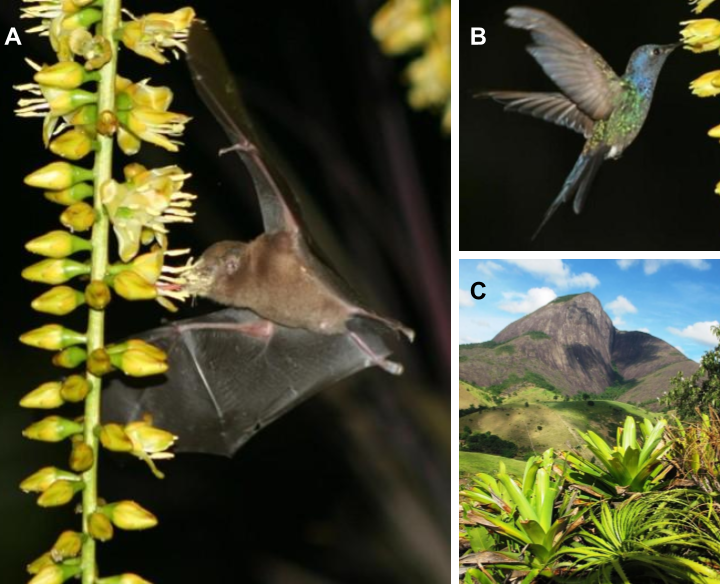
\includegraphics[width=90 mm]{figs/encholirium.png} 
 \caption{\textit{Encholirium horridum}. A and B - Flowers and pollinators (A – \textit{Glossophaga soricina} (Pallas, 1766) and C – \textit{Eupetomena macroura} (Gmelin, 1788); B - habit.}
  \label{encholirium}
\end{figure}


\begin{figure}
 \centering
  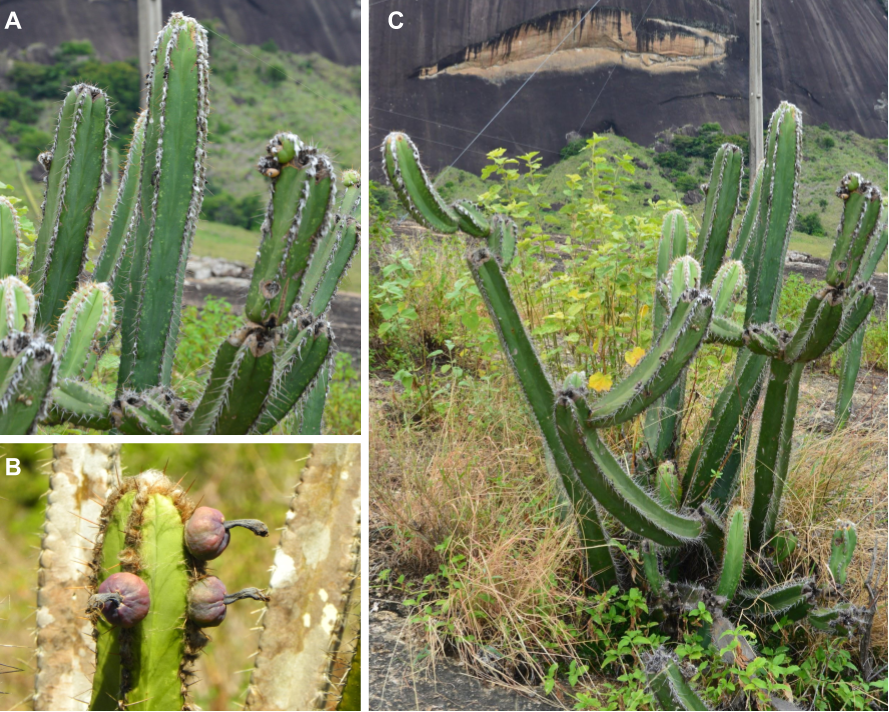
\includegraphics[width=90 mm]{figs/pilosocereus.png} 
  \caption{\textit{Pilosocereus brasiliensis}. A and C - habit and B - fruit.}
  \label{pilosocereus}
\end{figure}

\begin{figure}
  \centering
  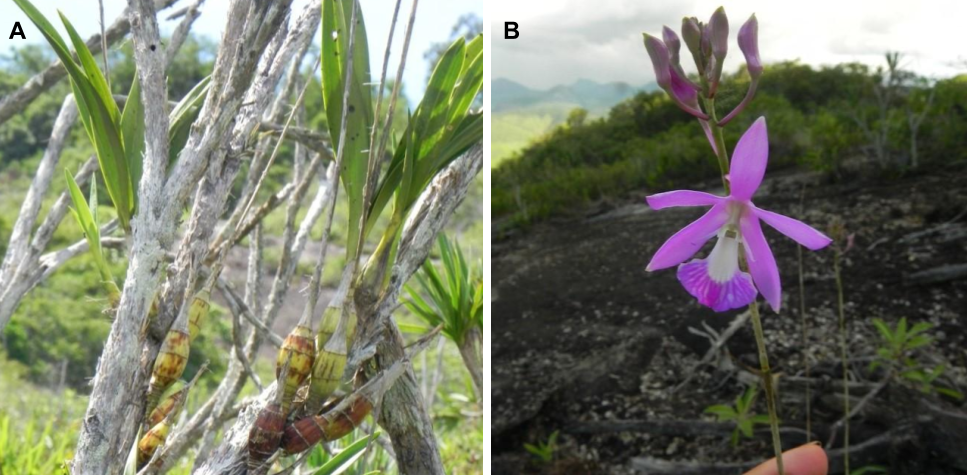
\includegraphics[width=90 mm]{figs/pseudo.png} 
  \caption{\textit{Pseudolaelia vellozicola}.  A - habit; B - flowers and flower buds.}
  \label{pseudo}
\end{figure}

\begin{figure}
  \centering
  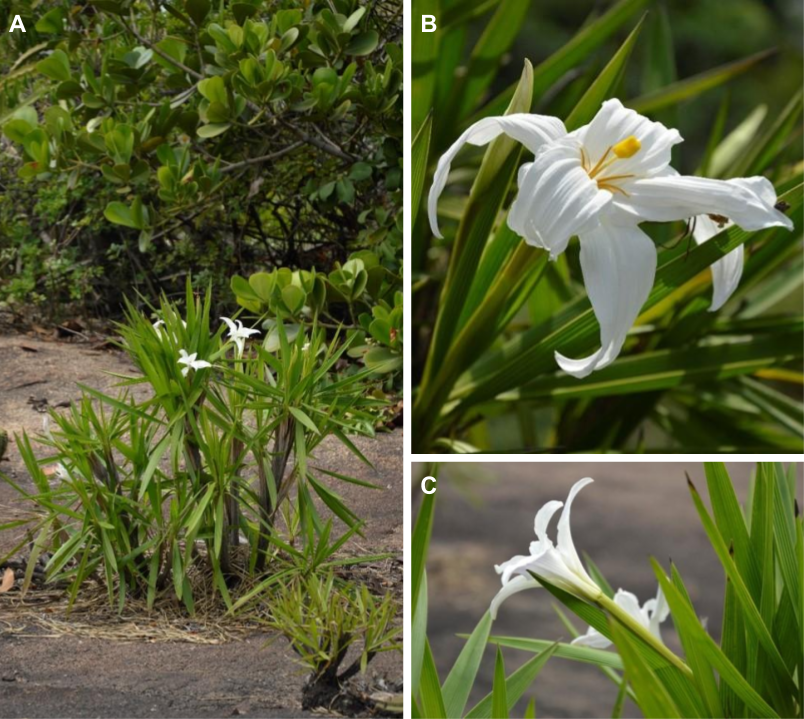
\includegraphics[width=90 mm]{figs/velozia.png} 
  \caption{\textit{Vellozia plicata}. A - habit, B and C - flower.}
 \label{velozia}
\end{figure}

\subsection{Study area}

The study area is located in the Atlântico Leste basin (7º 17 'to 20º 50' S and 36º 15 'to 47º 39' W) and São Francisco basin (9º 40 'to 19º 00' S and 36º40 'to 44º 00' W) (Figure \ref{bacias}), covering the so-called "sea of hills" area \citep{absaber1967DominiosMorfoclimaticosProvincias}. The São Francisco basin climate have the rainy season from November to January, contributing 53\% of the annual precipitation, while the driest period is from June to August \citep{mma-ministeriodomeioambiente2006CadernoRegiaoHidrografica}. The Atlântico Leste basin presents a warm and humid climate with relative humidity decreasing gradually towards the coast-continent \citep{mma-ministeriodomeioambiente2006AtlanticoSudesteCaderno}.

\begin{figure}
  \centering
  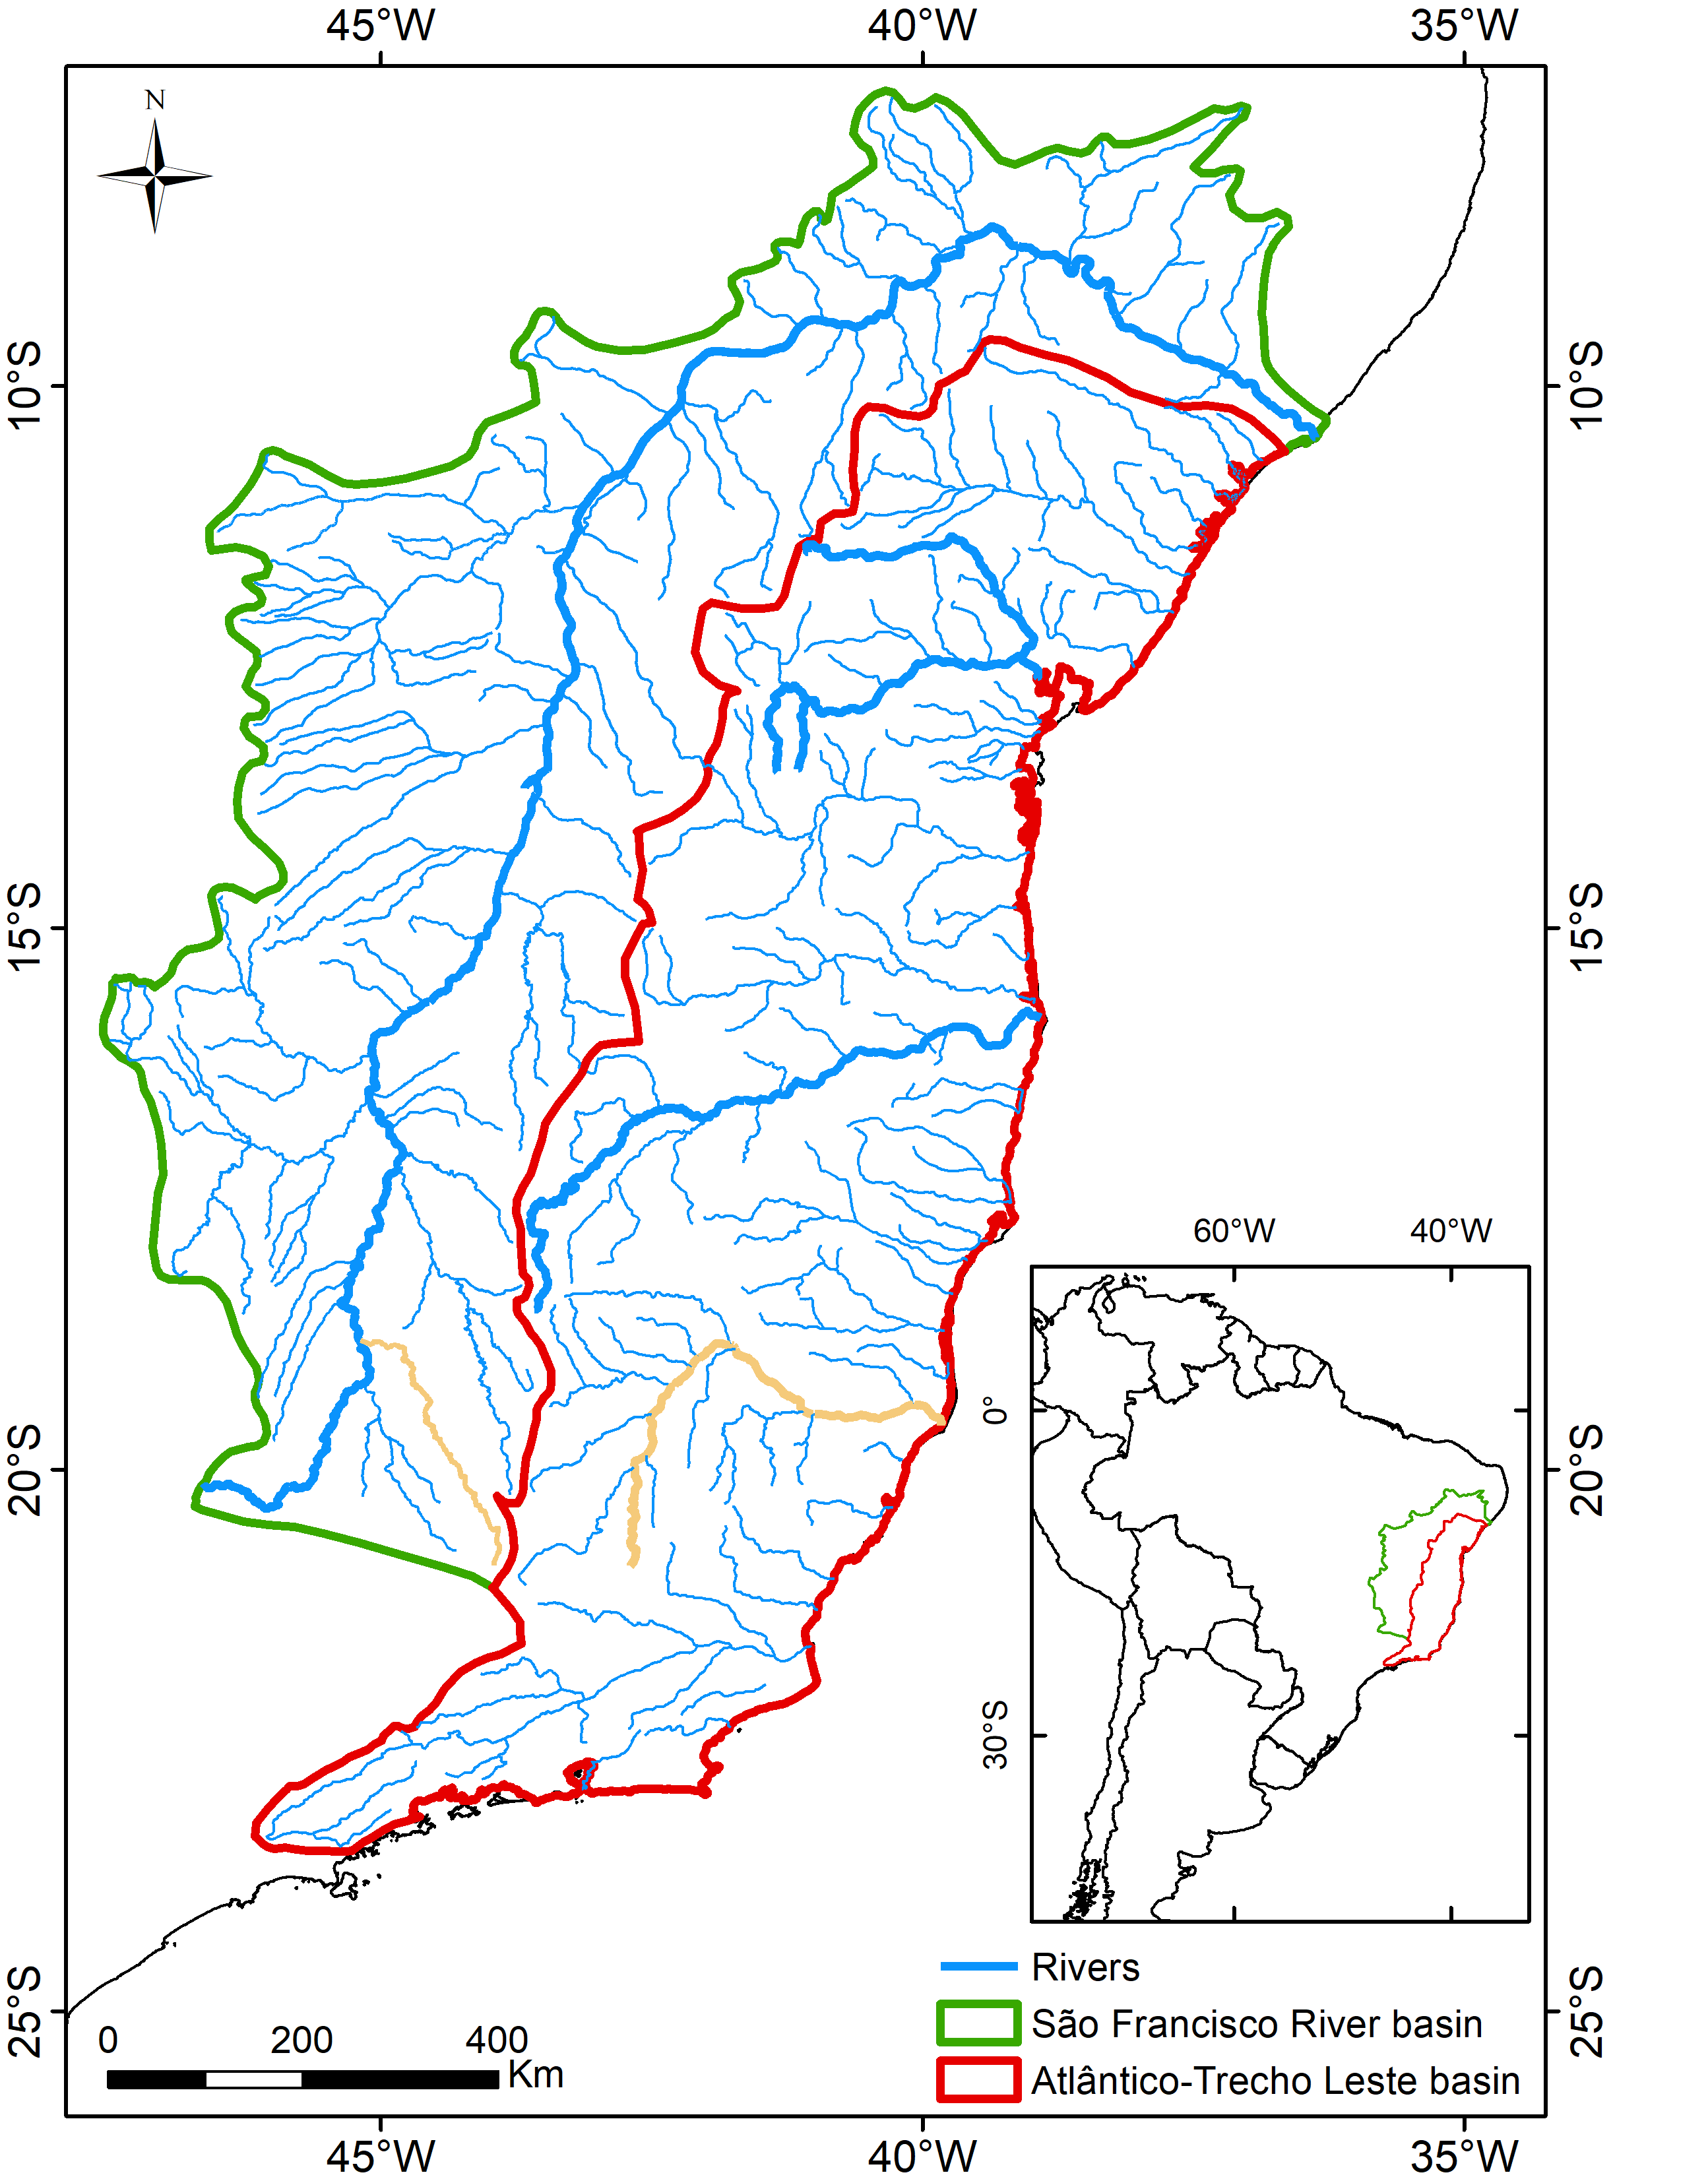
\includegraphics[width=90 mm]{figs/bacias.png} 
  \caption{Study area  with the São Francisco and Atlântico Leste hydrographic basins delimitation.}
 \label{bacias}
\end{figure}

\subsection{Obtaining and cleaning data}

The occurrence records of the species were obtained from GBIF databases - Global Biodiversity Information Facility (gbif.org), speciesLink (splink.org.br), and Reflora (reflora.jbrj.gov.br). The identification check was carried out by virtual consultation with the RB collection (jbrj.gov.br/jabot), where most of the samples are deposited. The doubtful records regarding the locality of collection were checked in specific literature and consulted to the specialists of each taxon. After the data was corrected, the records were reviewed with the help of the Google Earth Pro version 7.1.7 program. During data processing, dubious occurrences (\textit{i.e.} incomplete or uncertain location, repeated coordinates) and present on the same pixel were excluded. To reduce geographic location uncertainty, a review of the records was done with the help of the Google Earth Pro version 7.1.7 program. During data processing, dubious occurrences (\textit{i.e.}, incomplete or uncertain location, repeated coordinates). To reduce the spatial autocorrelation, only one point per pixel per species was used, resulting in points with a minimum distance of 1 km. At the end of the data cleaning, 54 records were used for \textit{Encholirium horridum}, 26 for \textit{Pilosocereus brasiliensis}, 60 for \textit{Pseudolaelia vellozicola} and 87 for \textit{Vellozia plicata}.

\subsection{Obtaining and selecting predictor variables}
The environmental variables used were obtained from the Worldclim 2 database \citep{fick2017WorldClimNew1km}, with spatial resolution of 30 arc-seconds ($\sim$1km). To eliminate the data collinearity, only the variables with a correlation lower than 0.7 were selected (i.e. minimum solar radiation, minimum temperature, maximum temperature, minimum water vapor pressure and minimum wind speed).

\subsection{Ecological niche modeling}
The modeling process that was performed in the R environment using the Model-R package \citep{sanchez-tapia2018ModelRFrameworkScalable}. To evaluate the models statistical performance, the k-fold \citep{fielding1997ReviewMethodsAssessment} partitioning method was used using four random partitions. To increase the number of models evaluated, this data partition was performed 5 times, thus totaling 20 models per species per algorithm (4 partitions x 5 runs). Since there are no points of absence of the species studied, 1000 randomly generated pseudo-absence points were used within a buffer, around the points of presence, with the mean distance between the points of presence. The model performance was evaluated by the True Skill Statistic (TSS) \citep{allouche2006AssessingAccuracySpecies}, using the threshold that maximizes the sum of sensitivity and specificity producing more accurate predictions \citep{jimenez-valverde2007ThresholdCriteriaConversion}. The algorithms used were Bioclim, Maxent, RandomForest (RF), Boosted regression trees (BRT) and Support Vector Machine (SVM). A consensus model (ensemble) was then developed, consisting of the mean of the models of all algorithms with TSS $\geq$ 0.7.

%\subsection{Niche overlap}

To assess distributional overlap based on ENMs, we used maps of binary presence/absence. The niche overlay was computed from predictions of species distributions with the modified Hellinger statistic (I), as proposed by \cite{warren_environmental_2008}. The statistic ranges from 0 (no overlap) to 1 (the distributions are identical). 

%%%%

%[doi:10.3390/insects10010033]

%To assess distributional overlap based on ENMs, we used maps of binary presence/absence as well as continuous occurrence probabilities. We used binary predictions, because this allowed us to determine which species co-occurred in areas of distributional overlap. However, since the use of continuous predictions has been recommended when estimating species richness [52], we calculated the sum of Reticulitermes species’ occurrence probabilities (Figure S4), and calculated joint and exclusive occurrence probabilities for each of the three species (Figure S5). For binary predictions, the approach of maximizing sensitivity and specificity has consistently performed better than other methods [53–55]. Thus, we used the True Skill Statistic (TSS = sensitivity + specificity − 1) [56] both as a model performance metric and to identify a threshold for converting continuous occurrence probabilities to binary classifications. The threshold was chosen based on maximizing the TSS, without risking under-prediction of presences (i.e., selecting the lowest threshold at which TSS is maximized). We used a threshold value of 0.2, where probability > 0.2 represented presence, and suitability ≤ 0.2 represented absence. We merged the three species’ binary maps by summing re-coded maps, where absence = 0, but presence was coded depending on species: R. flavipes = 4, R. virginicus = 2, and R. malletei = 1. This way, the sum of binary maps resulted in seven distinct categories: single-species areas (3 categories, with aforementioned scores); areas of two-species overlap (3 categories, scores of either 3, 5, or 6 depending on the identity of the species pair); and areas where all three species overlap (1 category, with a score of 7).

%%%%


\section{Results}
\label{results}

% TRECHO RETIRADO - PCA
\iffalse

\subsection{Principal Component Analysis}

Principal Component Analysis (PCA) based on the climate space studied concentrated 75.7\% of the total variation contained in the axes (PC1 = 42.3\% and PC2 = 33.4\%) (Figure 6). The variables that most contributed to the configuration of axis 1 (PC1) were temperature peaks (tmin and tmax) and precipitation (precip). Wind and radiation variables contributed less to axis 2 (PC2) (Table \ref{tab_pca}).

% For tables use
\begin{table}
% table caption is above the table
\caption{Principal Component Analysis (PCA) based on environmental space.  wind-world, tmin-world, tmax-world, srad-world, precip-world}
\label{tab_pca}       % Give a unique label
% For LaTeX tables use
\begin{tabular}{lll}
\hline\noalign{\smallskip}
first & second & third  \\
\noalign{\smallskip}\hline\noalign{\smallskip}
number & number & number \\
number & number & number \\
\noalign{\smallskip}\hline
\end{tabular}
\end{table}


% PCA Figure
\begin{figure}
 \centering
 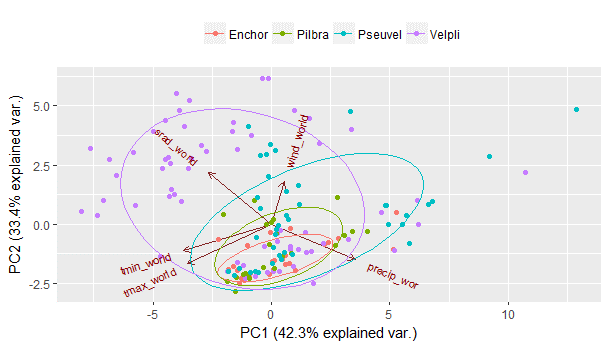
\includegraphics[width=80 mm]{figs/pca.png} 
 \caption{Principal Component Analysis (PCA)  based on environmental space shared by the species. Velpli: \textit{Vellozia plicata}; Pseuvel: \textit{Pseudolaelia vellozicola}; Pilbra: \textit{Pilosocereus brasiliensis}; Enchor: \textit{Encholirium horridum}. Srad-world: radiação solar; wind-world: velocidade do vento; tmin-world: temperature minima; tmax-world: temperature máxima; precip-world: precipitação}
  \label{pca}
\end{figure}

\fi

% FIM DO TRECHO RETIRADO DE PCA


\subsection{Ecological niche modeling}

The ecological niche models showed good predictability, considering that the algorithms presented good performance, with most of TSS values $\geq$ 0.7 and AUC $\geq$ 0.90  (Figure \ref{boxplot} and Table \ref{evaluate_summary}). The models also showed low omission and commission rates (For more details, see supplemental material). The Bioclim algorithm only performed well in the models of \textit{Encholirium horridum}.

% BOXPLOT
\begin{figure}
 \centering
 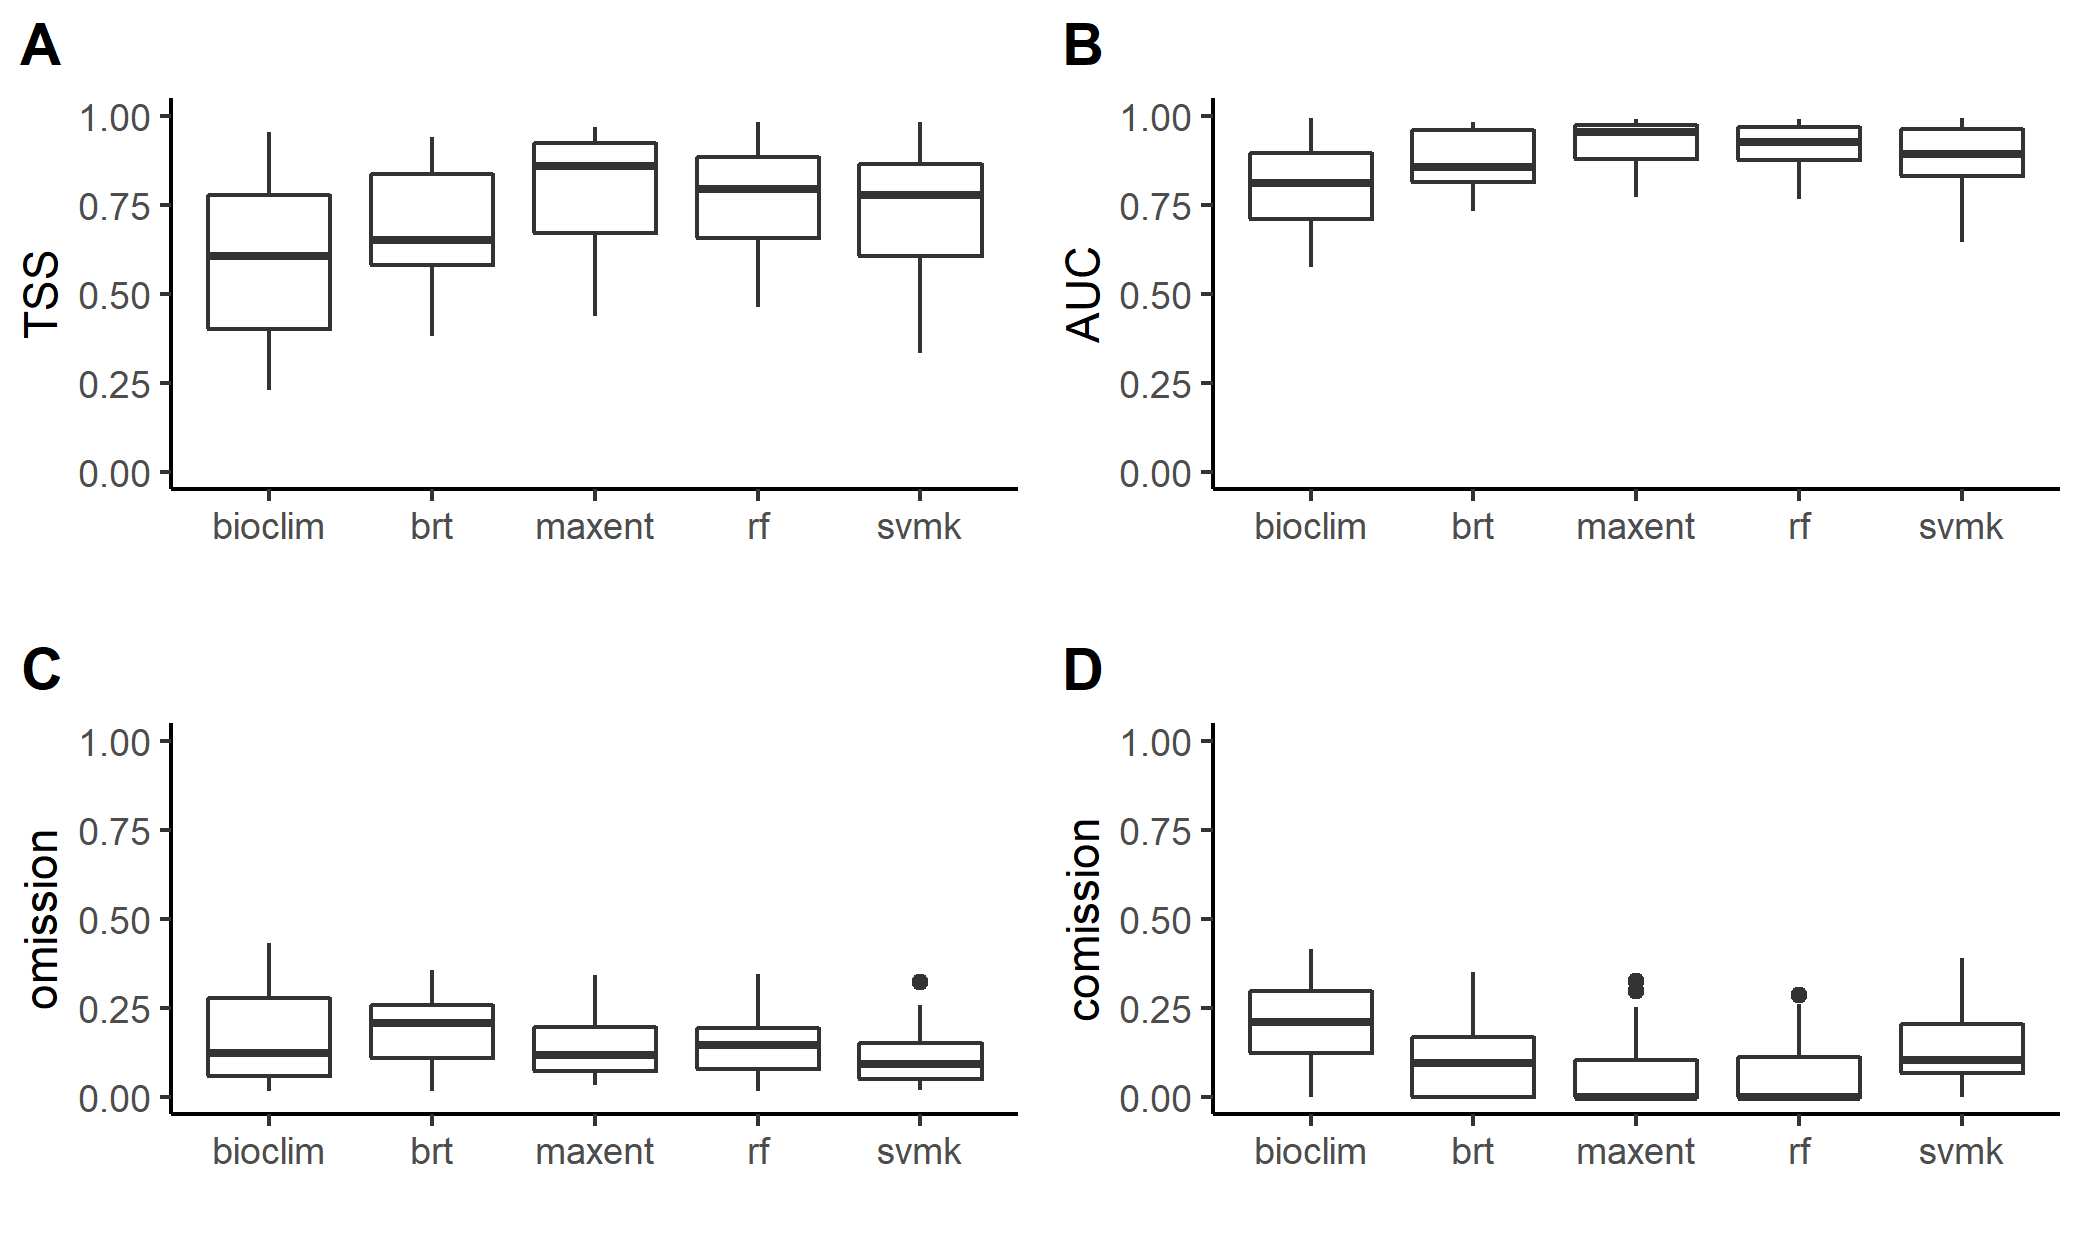
\includegraphics[width=90 mm]{figs/boxplot_tss_auc_OK.png} 
 \caption{Boxplot with TSS, AUC, omission and comission errors values. ö}
  \label{boxplot}
\end{figure}

%EVALUATE
\begin{table}[ht]
\label{evaluate_summary}
 \caption{Statistics for each partition of the algorithms used in creating the model.}
%\centering
\begin{tabular}{rllllll}
  \hline
 Species  & Algorithm & AUC & TSS & Omission & Comission \\ 
  \hline
 EncHor & bioclim & 0.92(0.05) & 0.82(0.09) & 0.04(0.02) & 0.12(0.07) \\ 
 EncHor & brt & 0.97(0.01) & 0.87(0.05) & 0.08(0.04) & 0.03(0.05) \\ 
 EncHor & maxent & 0.98(0.01) & 0.91(0.03) & 0.08(0.02) & 0(0) \\ 
 EncHor & rf & 0.97(0.01) & 0.88(0.05) & 0.09(0.05) & 0.02(0.04) \\ 
 EncHor & svmk & 0.96(0.01) & 0.86(0.05) & 0.06(0.03) & 0.08(0.05) \\ 
 PilBra & bioclim & 0.85(0.1) & 0.7(0.2) & 0.07(0.02) & 0.18(0.13) \\ 
 PilBra & maxent & 0.97(0.01) & 0.93(0.02) & 0.06(0.01) & 0(0) \\ 
 PilBra & rf & 0.96(0.02) & 0.89(0.06) & 0.08(0.04) & 0.02(0.05) \\ 
 PilBra & svmk & 0.92(0.07) & 0.84(0.13) & 0.07(0.05) & 0.07(0.1) \\ 
PseVel & bioclim & 0.78(0.06) & 0.55(0.11) & 0.24(0.04) & 0.2(0.1) \\ 
PseVel & brt & 0.84(0.04) & 0.66(0.08) & 0.24(0.05) & 0.05(0.07) \\ 
 PseVel & maxent & 0.92(0.03) & 0.77(0.05) & 0.16(0.04) & 0.04(0.05) \\ 
PseVel & rf & 0.89(0.03) & 0.73(0.07) & 0.18(0.04) & 0.05(0.07) \\ 
 PseVel & svmk & 0.88(0.06) & 0.73(0.1) & 0.12(0.06) & 0.13(0.08) \\ 
VelPli & bioclim & 0.65(0.05) & 0.31(0.07) & 0.34(0.05) & 0.32(0.11) \\ 
VelPli & brt & 0.8(0.04) & 0.53(0.08) & 0.24(0.06) & 0.2(0.08) \\ 
 VelPli & maxent & 0.83(0.04) & 0.55(0.07) & 0.24(0.06) & 0.17(0.09) \\ 
 VelPli & rf & 0.85(0.04) & 0.59(0.07) & 0.23(0.05) & 0.15(0.09) \\ 
  VelPli & svmk & 0.79(0.07) & 0.53(0.11) & 0.18(0.05) & 0.26(0.08) \\ 
   \hline
\end{tabular}
\end{table}


%The most suitable region of the four species is within the limits of the East Atlantic basin and the occurrence records (except for \textit{Vellozia plicata}) are restricted to the same basin (Figure \ref{mod1} and \ref{mod2}).

The \textit{Encholirium horridum}  model's  was restricted to the Atlântico Leste basin, presenting a small region of high suitability in south central region of this basin (Figure \ref{mod1}A), with an area of 129,331 km$^{2}$ (7\%) along the study area. The algorithms showed excellent performance values,with mean of AUC 0.92 to 0.98 and TSS 0.82 to 0.91 (Table \ref{evaluate_summary}). 

\textit{Pilosocereus brasiliensis} has few records of herbarium occurrence and its model also is restricted to the Atlântico Leste basin, where it presented regions of high suitability, with an area of 154,438 km$^{2}$ (8\%) along the study area. Records were obtained from Espírito Santo, eastern Minas Gerais and one north of Rio de Janeiro state. Its model covers the states of Rio de Janeiro, Minas Gerais, Espírito Santo, southern Bahia state (Figure \ref{mod1}B) and showed good performance values, AUC from 0.85 to 0.97 and TSS from 0.70 to 0.93 (Table \ref{evaluate_summary}).

\textit{Pseudolaelia vellozicola} has its distribution restricted to the Atlântico Leste basin, in the states of Rio de Janeiro, Espírito Santo, Minas Gerais and Bahia (Figure \ref{mod2}A), with an area of 312,027 km$^{2}$ (16\%) along the study area. Most of your model in these states has a high suitability value. The model of this species presented good performance values, AUC from 0.78 to 0.92 and TSS from 0.55 to 0.73 (Table \ref{evaluate_summary}). 
%It was also possible to observe occurrence points right in the division line between the two basins, where there is a linear distribution along the Espinhaço Chain, in Minas Gerais state (Figure ).

The \textit{Vellozia plicata} model is present in both basins, even at low suitability in the São Francisco basin (Figure \ref{mod2}B), with an area of 502,575 km$^{2}$ (26\%) along the study area. Among the taxa studied here, this species has the largest area of occurrence, reaching the inselbergues of the Northeast region, in the Caatinga biome. It is also possible to observe that its model covered the Serra da Mantiqueira region, south of the Atlântico Leste basin in the São Paulo state. Moreover, the models presents similar performance values, AUC from 0.65 to 0.85 and TSS 0.31 to 0.59 (Table \ref{evaluate_summary}).



% mod1
\begin{figure}
 \centering
 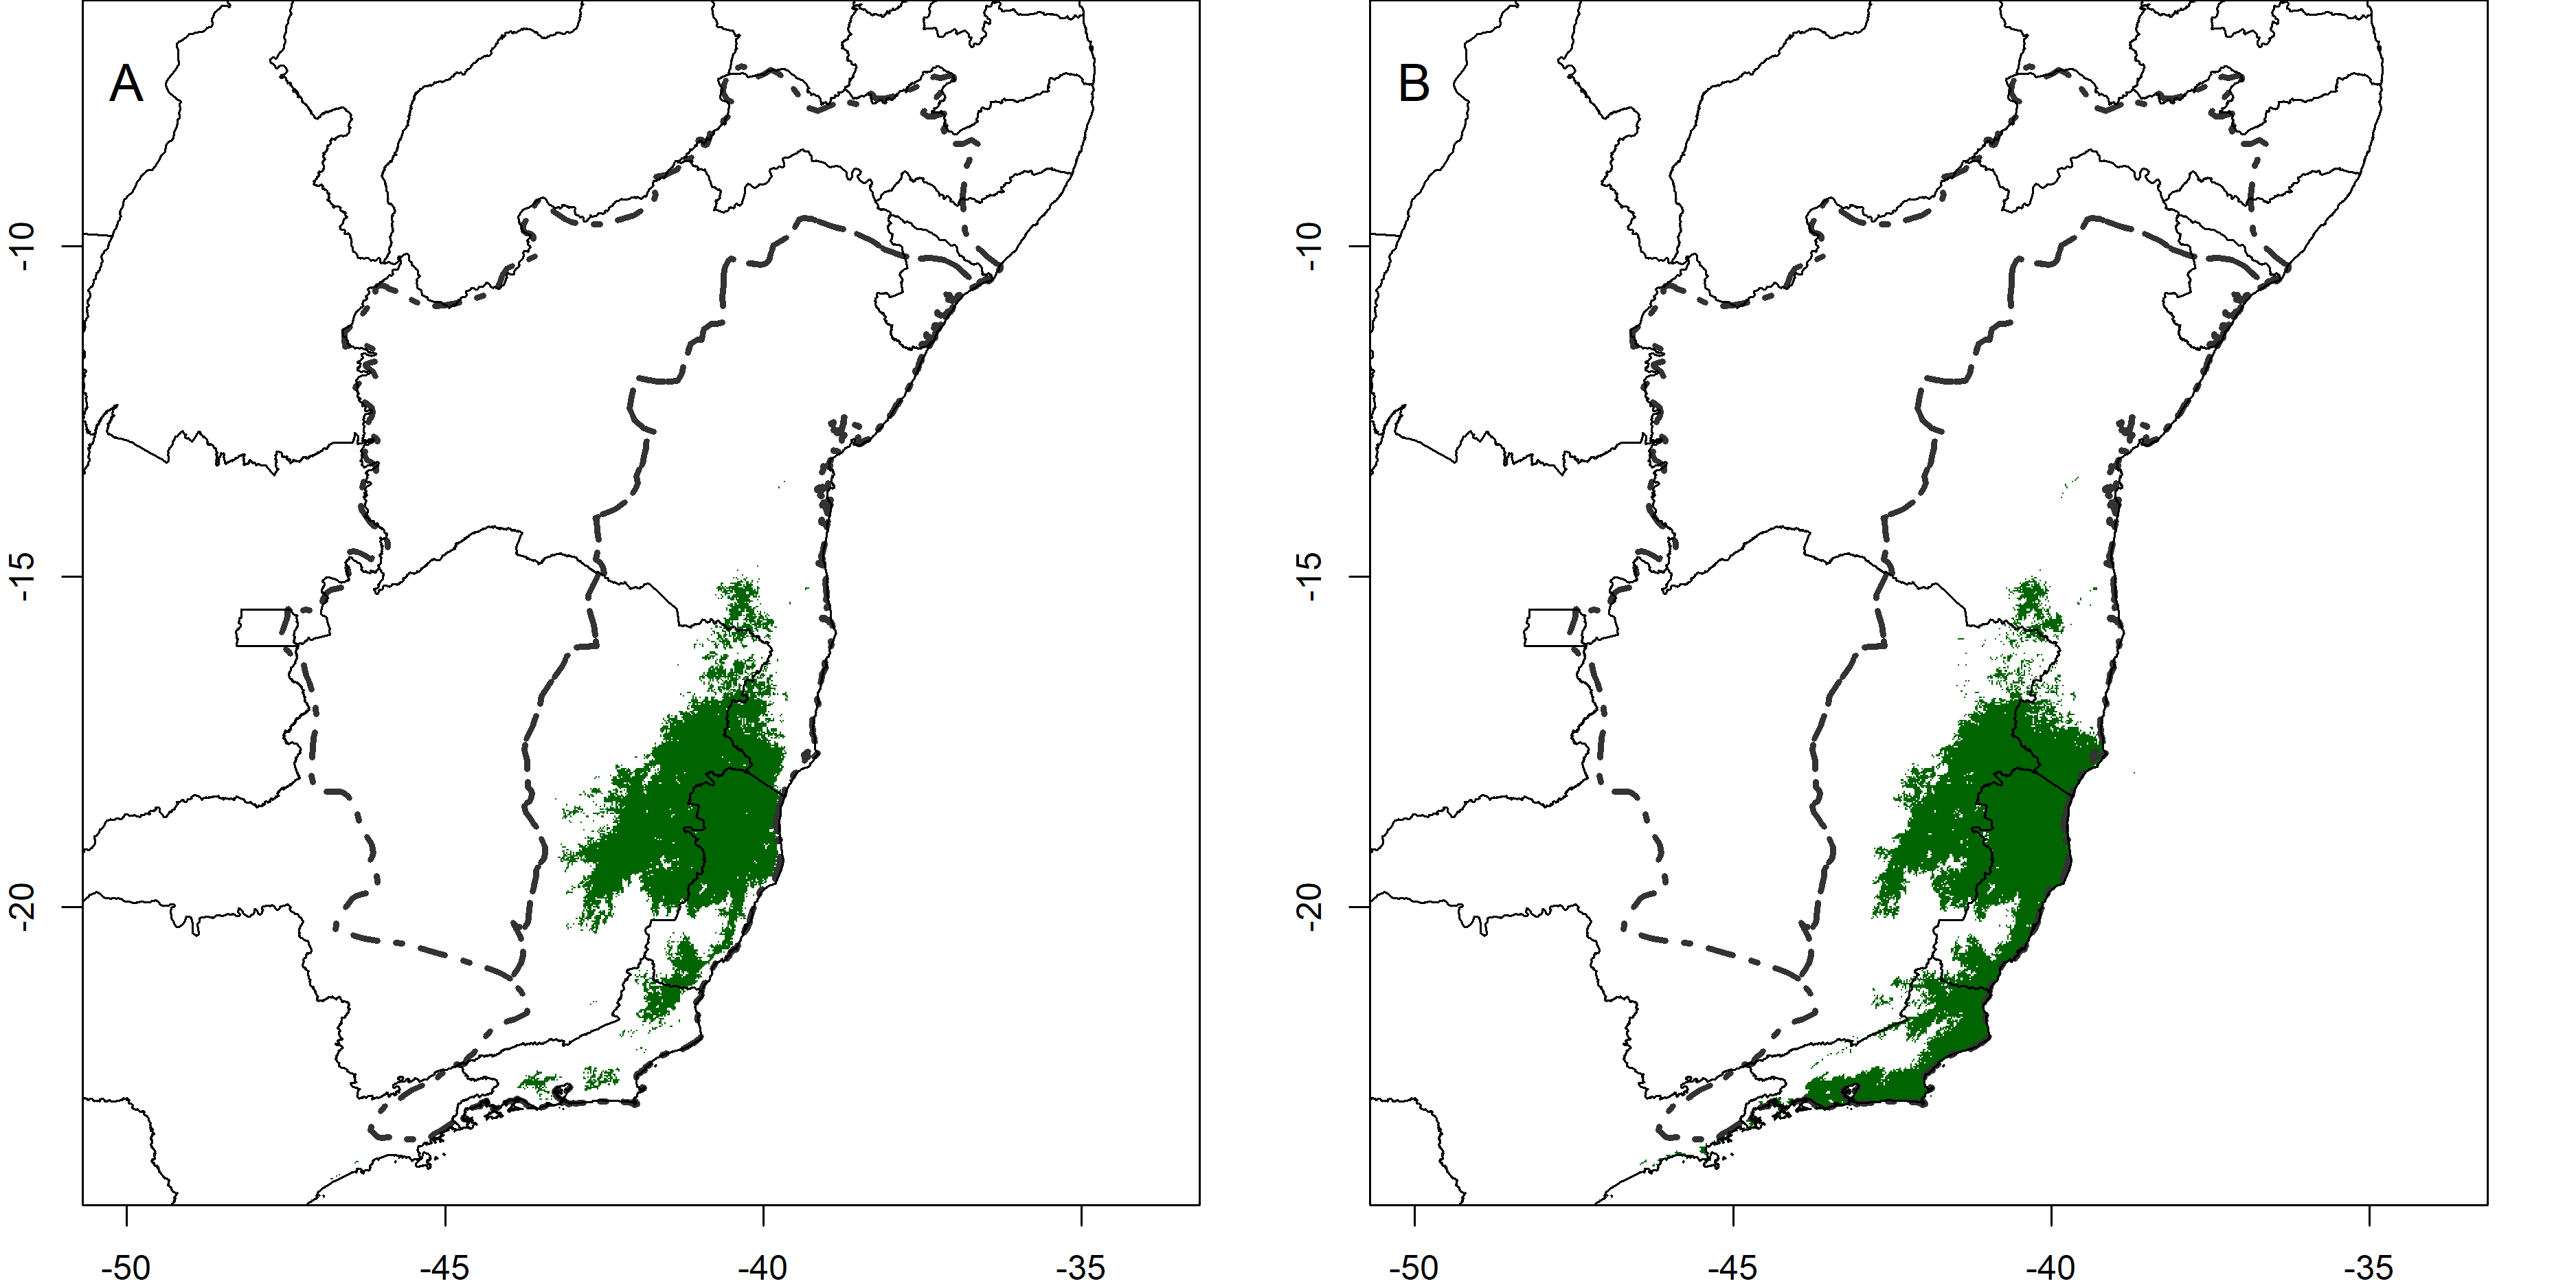
\includegraphics[width=90 mm]{figs/mod1.png} 
 \caption{Distribution of environmental suitability values for occurrence of (A) \textit{Encholirium horridum} L.B.Sm. and (B) \textit{Pilosocereus brasiliensis} (Buining \& Brederoo) Zappi. The dotted line is the boundary of the eastern Atlantic and São Francisco basins. The solid line is the limits of the Brazilian states.}
  \label{mod1}
\end{figure}

% mod2
\begin{figure}
 \centering
 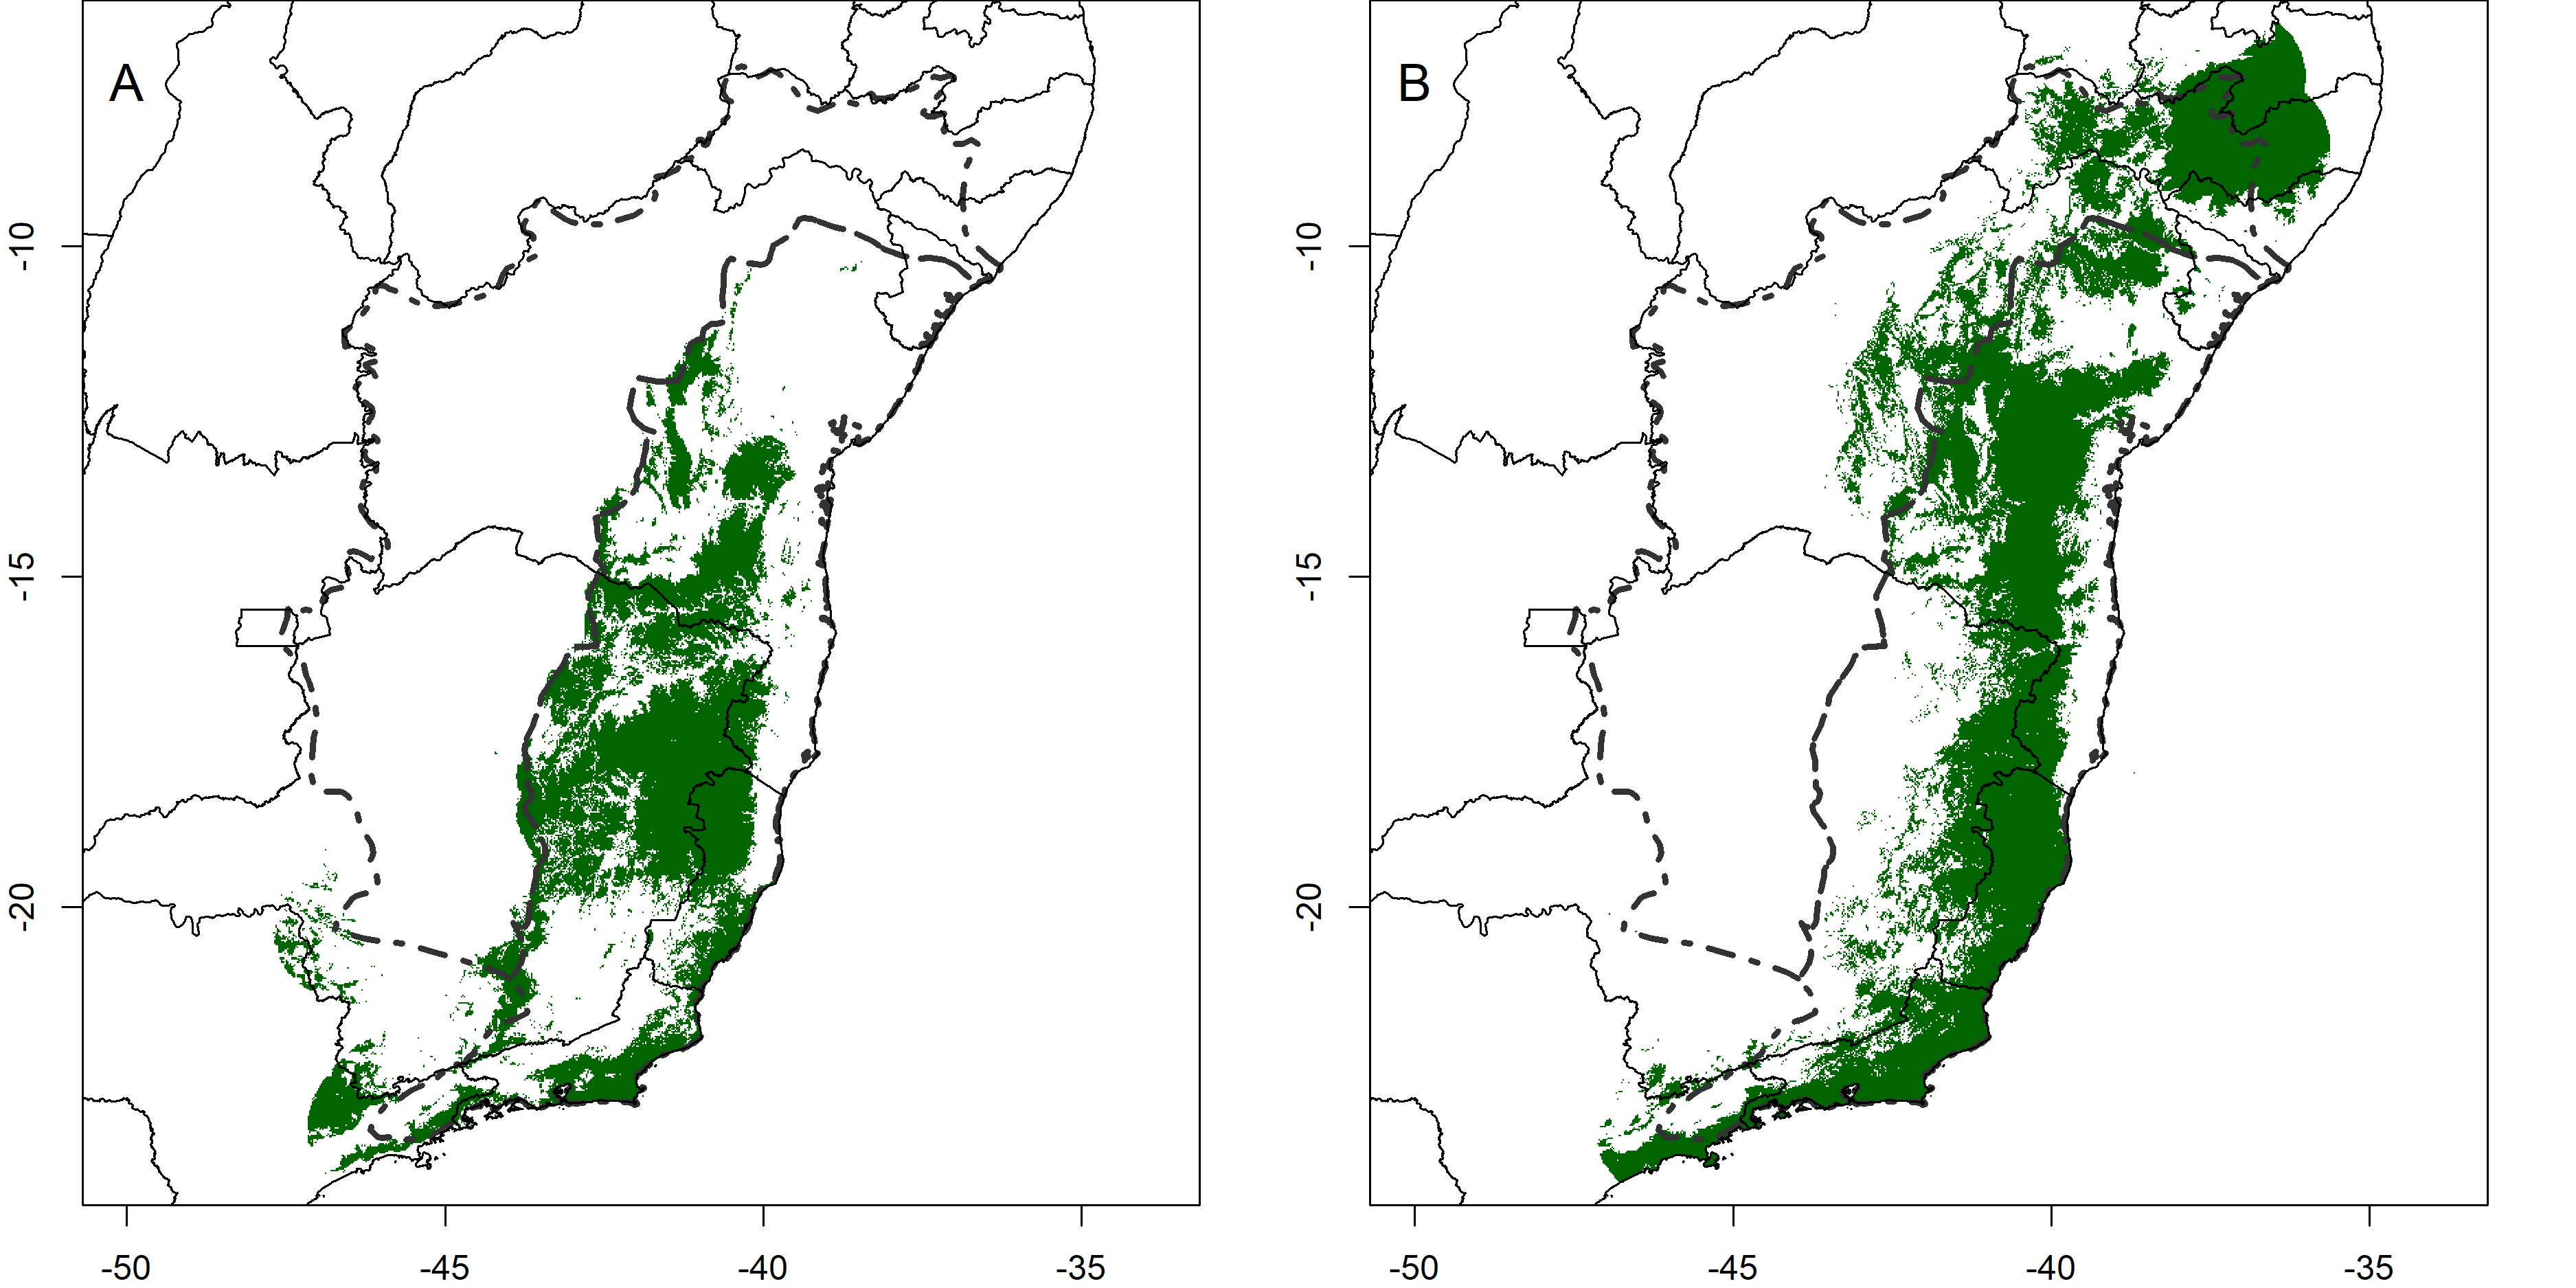
\includegraphics[width=90 mm]{figs/mod2.png} 
 \caption{Distribution of environmental suitability values for occurrence of (A)  \textit{Pseudolaelia vellozicola} (Hoehne) Porto \& Brade and (B) \textit{Vellozia plicata} Mart. The dotted line is the boundary of the eastern Atlantic and São Francisco basins. The solid line is the limits of the Brazilian states.}
  \label{mod2}
\end{figure}


%\subsection{Niche overlap}

Among the four inselbergues plants, the local realized niches of \textit{Encholirium horridum} and \textit{Pilosocereus brasiliensis} were most similar (overlap = 0.79, Table \ref{tab_nicheoverlap}), and local realized niches of \textit{Encholirium horridum} and \textit{Vellozia plicata} were most dissimilar (Table \ref{tab_nicheoverlap}).

% NICHEOVERLAP TABLE
\begin{table}[ht]
\caption{Niche overlap between four inselbergue plant species. enc = \textit{Encholirium horridum} ; pil = \textit{Pilosocereus brasiliensis} ; pse = \textit{Pseudolaelia vellozicola} ; vel = \textit{Vellozia plicata}.}
\label{tab_nicheoverlap} 
\centering
\begin{tabular}{cccc}
  \hline
 & enc & pil & pse \\ 
  \hline
pil & 0.79 &      &  \\ 
pse & 0.46 & 0.46 &  \\ 
vel & 0.41 & 0.47 & 0.45 \\ 
   \hline
\end{tabular}
\end{table}

\begin{table}[ht]
\caption{Niche overlap between four inselbergue plant species. enc = \textit{Encholirium horridum} ; pil = \textit{Pilosocereus brasiliensis} ; pse = \textit{Pseudolaelia vellozicola} ; vel = \textit{Vellozia plicata}.}
\label{tab_nicheoverlap} 
\centering
\begin{tabular}{cccc}
  \hline
Sítios	&	SBO_500	&	SBO_800	&	SLO_500	\\
  \hline
SBO\_800	&	0.44	&		&		\\
SLO\_500	&	0.54	&	0.33	&		\\
SLO\_800	&	0.23	&	0.22	&	0.28	\\
SPL\_500	&	0.65	&	0.32	&	0.59	\\
SPL\_800	&	0.29	&	0.34	&	0.29	\\
  \hline
\end{tabular}
\end{table}

The area with the greatest suitability for the four species studied was in the central-eastern region of the East Atlantic basin (Figure \ref{riq}). Important areas were also observed in the forests to the southeast of the state of Espírito Santo and the mountain region of Rio de Janeiro. In the Chapada Diamantina region, in central Bahia, they presented areas with suitability only for \textit{Pseudolaelia vellozicola} and \textit{Vellozia plicata}.

\begin{figure}
 \centering
 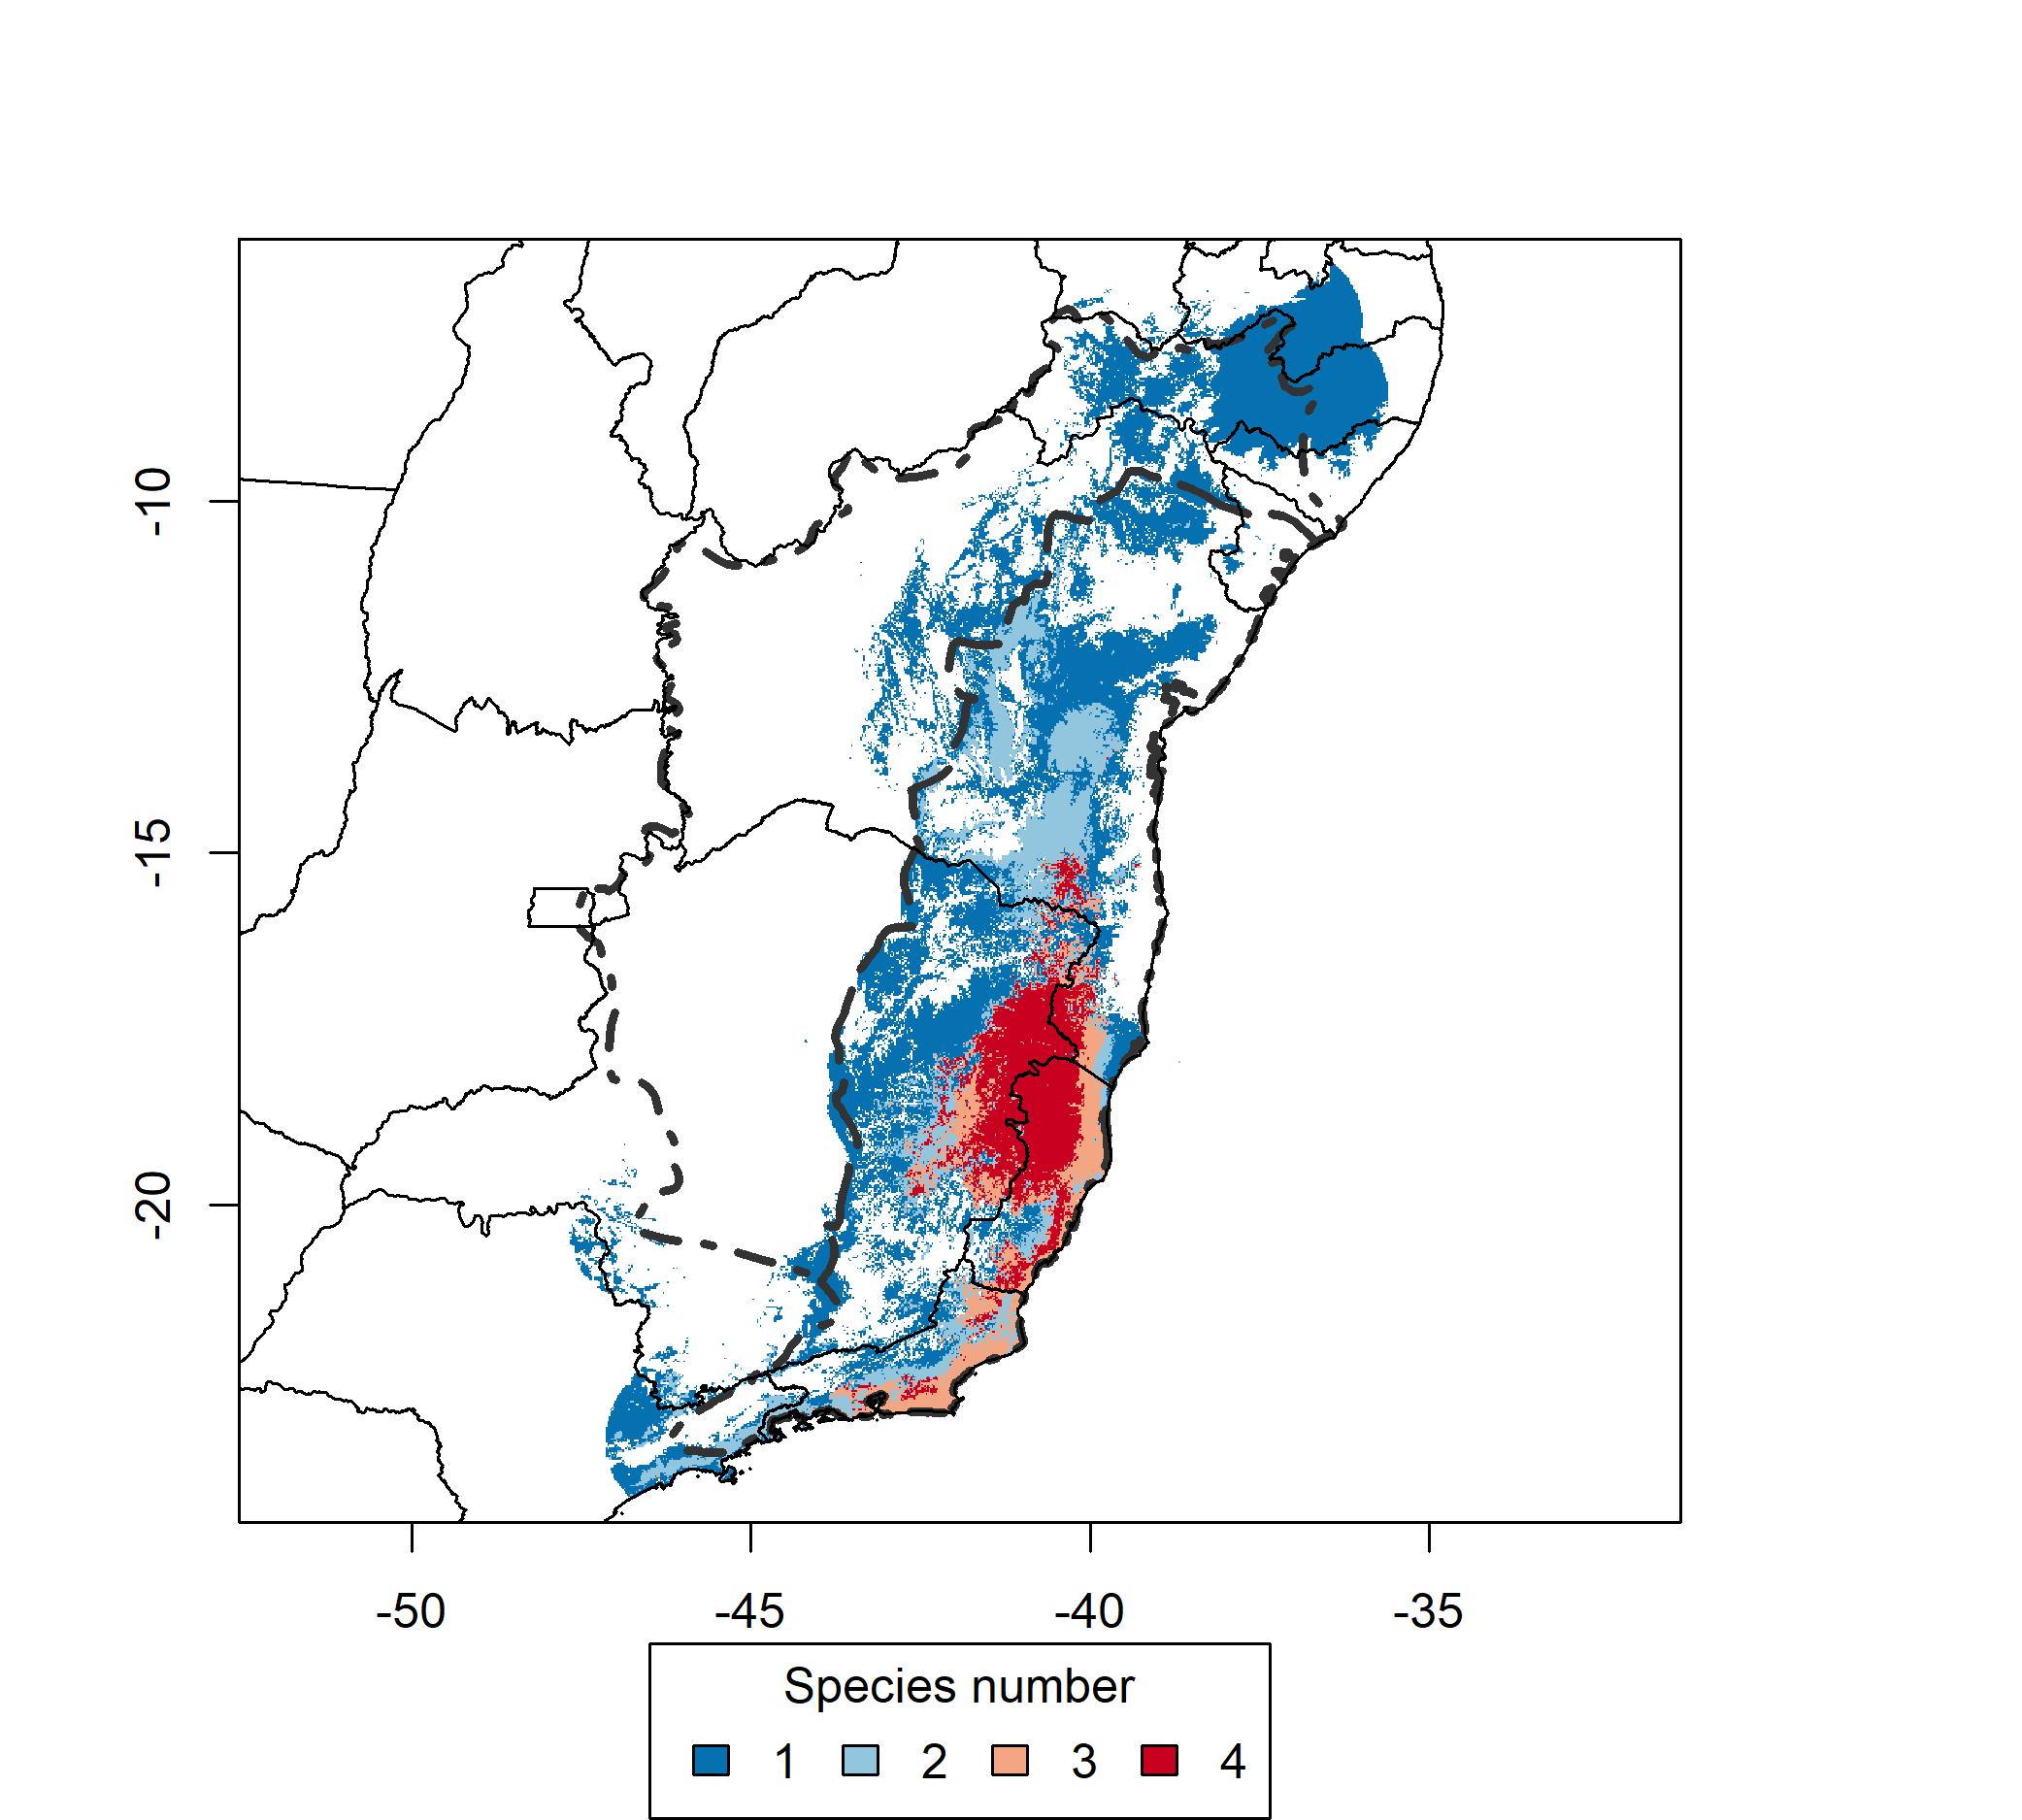
\includegraphics[width=90 mm]{figs/riq_bin.png} 
 \caption{Potential richness of the four species studied. The dotted line is the boundary of the eastern Atlantic and São Francisco basins. The solid line is the limits of the Brazilian states. ö}
  \label{riq}
\end{figure}

\subsection{Species conservation}

\textit{Encholirium horridum} is present in three protected areas, but no record of occurrence has been found within the full protected conservation unit. No occurrence records were found within the full protection conservation unit. However, there are many Protected Areas that have high environmental suitability, but no inselberges and without the substrate there is no occurrence of species. The overlap of the models with high suitability values of the species in the central eastern Atlantic basin and extending to a southern stripe closest to the coast. 

\textit{Pilosocereus brasiliensis} . Records were found in the APA Morro do Leme; Parque Nacional da Floresta da Tijuca; APA Waldeir Gonçalves - Serra do Itaóca. It was possible to observe areas of high suitability within Protected Areas that do not have records of occurrence of the species, they are: APA da Bacia do Rio São João - Mico Leão e APA do Pico do Goiapaba-Açu.

There are \textit{Pseudolaelia vellozicola} records in the following Protected Areas: APA Alto do Mucuri; Parque Estadual do Rio Preto; APA Águas Vertentes; Parque Estadual Serra Nova; Parque Natural Municipal Chácara Von Schilgen; Parque Estadual da Fonte Grande; Parque Estadual do Forno Grande; MONA dos Pontões Capixabas; Parque Municipal Morro da Pescaria. It was possible to observe high suitability areas within Protected Areas that do not have records of occurrence of the species, they are: APA da Bacia do Rio São João - Mico Leão; APA de Campinas; Parque Nacional das Sempre Vivas; Parque Estadual da Serra do Cabral, this UC being the only one outside the Atlântico Leste basin.

\textit{Vellozia plicata} is the species with the largest number of records and the widest geographical distribution, reaching the inselbergues of the north of the Rio de Janeiro state, in the domain of the Atlantic Forest to Paraíba, in the Caatinga biome. It is also the species with the largest number of records within Conservation Unit (UC), occurs in APA da Lagoa Itaparica; ARIE Serra do Orobó; APA da Serra do Barbado; Parque Estadual da Fonte Grande; Parque Estadual Serra do Brigadeiro; APA Waldeir Gonçalves - Serra do Itaóca. It was possible to observe areas of high suitability within Protected Areas that do not have records of occurrence of the species, they are: APA da Bacia do Rio São João - Mico-Leão-Dourado; REBIO de Sooretama; Parque Estadual de Sete Salões.


\section{Discussion}

\subsection{Ecological niche modeling}

The delimitation of the Atlântico Leste and São Francisco basins seems to have an influence on the geographic distribution of the species studied here, acting as barriers. Because, in addition to the occurrence points being restricted to the basins, the models indicated areas of suitability mainly in the East Atlantic basin. However, other factors must be taken into account, such as the presence of the substrate (i.e. existence of inselbergs), climate, pollinator and disperser.

Many species of Velloziaceae occur in inselbergs, and many of them are tolerant to desiccation and adapted to severe environmental conditions \citep{porembski2000InvasibilityTropicalGranite}. Among the groups under study, Vellozia is the oldest group \citep{mello-silva2011FiveVicariousGenera} and \textit{Vellozia plicata} is the species with the widest distribution, with records of occurrence in both basins. This can be explained by the time that it is in the ecosystem, which allows the expansion of its area of occurrence. In addition, \textit{V. plicata} records were found not only in granite / gneiss, but also in limestone rocks and rupestrian fields, in the Caatinga domain, being the only species found in these three types of substrate, presenting characteristics of a generalist species.

\textit{Pseudolaelia} has a restricted occurrence throughout eastern Brazil and has a distribution pattern similar to the other genera studied, including \textit{Encholirium} \citep{meninineto2012BiogeographyConservationStatus}. The distribution region along the Espinhaço Chain in Minas Gerais state, was considered an area of species richness, diversity and endemism for the genre \citep{meninineto2012BiogeographyConservationStatus}. The models obtained for \textit{Pseudolaelia vellozicola} demonstrate the existence of a small region (Serra do Cabral) of high suitability in the São Francisco basin. This region is located between the basins of the rivers Velhas and Jequitaí, being considered an area of rupestrian field disjunct to the Espinhaço complex. The absence of records of \textit{P. vellozicola} in this area may not be due to the lack of collections, but because Serra do Cabral is located outside the East Atlantic basin, which may be acting as a barrier in dispersion. \textit{P. vellozicola} occurs in rupestrian fields and in granite / gneiss, in the domain of the Cerrado, thus increasing its distribution area.

\textit{Pseudolaelia vellozicola} has an extremely variable floral morphology. In addition to being the species with the greatest geographic distribution within the genus, it is the one with the highest degree of genetic polymorphism \citep{meninineto2013TaxonomicRevisionPseudolaelia}. This variation can be explained by the fact that the inselbergs can act as isolated islands, reducing the gene flow. With low gene flow, morphological differentiation can occur through isolation, this differentiation reinforces the need for greater care in the description of new species and their geographical delimitation \citep{barthlott2000WhyStudyInselbergs,meninineto2012BiogeographyConservationStatus}.

The Cactaceae family represents the second in order of size among vascular plants endemic in the Americas, with Bromeliaceae in first place \citep{zappi2011PlanoAcaoNacional}. The genus Pilosocereus is the one with the greatest representativeness in Brazil \citep{zappi1994PilosocereusCactaceaeGenus}. However, \textit{P. brasiliensis} has few records, this may be due not only to the difficulty of collection, or low taxonomic interest in the species, but also because the inselbergs in general are poorly collected \citep{depaula2016SugarLoafLand, porembski2007TropicalInselbergsHabitat}. Due to the small amount of registration available, the model generated should be taken with caution, knowing that one of the fundamental characteristics that contribute to an ecologically sensitive model is the number and quality of available records.

The model obtained for \textit{Encholirium horridum} shows a region of high suitability to the east of the state of Minas Gerais on the border with Espírito Santo, but with no occurrence records. In this region there is a large chain of inselbergs, an area called “sea of hills” \citep{absaber1967DominiosMorfoclimaticosProvincias}, and the absence of points of occurrence may indicate a lack of collection. The northwestern landscape of Espírito Santo is characterized by a concentration of inselbergs in the formation of a mountain range. In this region, populations of E. horridum are found closer to each other, allowing connectivity, and where populations have greater genetic diversity \citep{hmeljevski2017PlantPopulationsDistinct}. 

The region to the east of Espírito Santo doesn't have inselbergs, that is, it has climatic suitability, but it doesn't have the substrate required by the species. The record of Encholirium horridum further north in the state of Rio de Janeiro and south of Espírito Santo, indicates the presence of the substrate, even with low climatic suitability. It is also possible to observe points of occurrence more distant from the region of greater suitability. These extremes of occurrence are located in inselbergs geographically more isolated in the landscape, south of Bahia, east of Minas Gerais and north of Rio de Janeiro. These more isolated populations have less gene flow, are experiencing declines in their sizes, resulting in loss of genetic diversity, accompanied by greater differentiation between populations \citep{hmeljevski2017PlantPopulationsDistinct}.

\subsection{Distribution Patterns}

\subsection{Species conservation}

%[Isso aqui parece introdução/justificativa ö]

%Inselbergues abrigam uma vegetação bastante peculiar que se desenvolve em condições adversas (De Paula et al., 2016; Porembski, 2007). As famílias das espécies aqui em estudo são, em geral, as de maior riqueza específica em trabalhos sobre a flora de inselbergues (De Paula et al., 2017a; Gomes \& Alves, 2009; Porembski et al., 1998; Porembski; Barthlott, 2000) e possuem diferentes estratégias adaptativas (e.g. fisiológicas, morfológicas) que possibilitam a sobrevivência em condições extremas (DE Paula et al., 2016; Menini Neto \& Forzza, 2012).  A matriz florestal também é um componente de grande influência na variação das comunidades de inselbergues do sudeste brasileiro, afetando especialmente  a capacidade de dispersão das espécies (Porembski et al., 2000).  

%[ate aqui]
 
\textit{Encholirium horridum} and \textit{P. brasiliensis}, may have a more restricted distribution than \textit{V. plicata} and \textit{P. vellozicola} due to the type of climate they are adapted to. The absence of these species in the south of Rio de Janeiro can be explained because in this area the "archipelago of inselbergs" has more humid characteristics, sheltering a distinct community, and with greater annual precipitation than regions of the center / north of Espírito Santo \citep{oliveira-filho2000PatternsFloristicDifferentiation}. \citet{depaula2016SugarLoafLand} points to the climate as the main influence on the distribution of bromeliads. Encholirium horridum is a characteristic species of drier areas, being the only one that doesn't have suitability in the south of the state of Espírito Santo and Rio de Janeiro.
 
\textit{Pilosocereus brasiliensis} is pollinated predominantly by bats \citep{lucena2007FenologiaBiologiaPolinizacao, taylor2004CactiEasternBrazil}, being the only species in this study that has berry type fruit, dispersed by bats and birds, presenting restricted distribution to inselbergs from Bahia, Espírito Santo, Minas Gerais and Rio de Janeiro \citep{bfg2018BrazilianFlora2020}. \textit{Encholirium horridum} is pollinated by bats and hummingbirds and the dispersion of its seeds is possibly due to the wind, but over short distances (Hmeljevski, 2013) \citep{hmeljevski2015PatternsGeneFlow}. It has a more restricted distribution than \citep{Pilosocereus brasiliensis} and a smaller climatic niche and shared with all other species, despite having a larger number of records, indicating that it also has a broader ecological niche.

\textit{Vellozia plicata}, despite having a restricted dispersion mechanism \citep{franceschinelli2006GeneticDiversityTwo, jacobi2007PollinationTwoSpecies}, is the species with the greatest geographical distribution and the widest climatic niche among the studied species, indicating characteristics of a generalist taxon. \textit{Pseudolaelia vellozicola} is dispersed by the wind and may be rupicolous or epiphytic over different species of \textit{Vellozia} (Menini Neto, 2013), being the only taxon in this study that does not share its entire climatic niche with \textit{Vellozia plicata}.

Dispersion is one of the factors of great influence in the colonization of new environments and also in the explanation of the phylogenetic structure \citep{parmentier2009ImpactEcologicalDifferentiation}. In the present study, \textit{Encholirium horridum}, \textit{Pilosocereus brasiliensis} and \textit{Vellozia plicata}, have a restricted dispersion mechanism, however, \textit{V. plicata} has a distribution contrary to what its dispersion mechanism suggests. This may be because Vellozia is an older group, had more time to colonize new places, and also, the connection between the flora of the inselbergs in the past, which facilitated its expansion, today with the increased fragmentation of the matrix, reduces the possibility colonization of these islands, increasing the isolation between them \citep{mello-silva2011FiveVicariousGenera, safford1999BrazilianParamosIntroduction}.

%\subsection{Niche overlap}

%The niche overlap...

\subsection{Conservação das espécies}

Inselbergs' richness and endemism are widely recognized and frequently cited, many taxa are restricted to certain altitudinal bands, common characteristics of species from the Bromeliaceae, Orchidaceae and Velloziaceae families \citep{barbara2007PopulationDifferentiationSpecies,giulietti2005BiodiversityConservationPlants, martinelli1989CamposAltitude, mello-silva2011FiveVicariousGenera, meninineto2012BiogeographyConservationStatus,porembski2007TropicalInselbergsHabitat, porembski1998DiversityEcologySaxicolous}. The greatest threat to species in these environments is habitat degradation, due to some stochastic event or by anthropic action, through fire or granite extraction, with the main consequence of decreasing populations \citep{forzza1998EncholiriumUmGenero}.

All species studied here have records in Conservation Units. However, the number of records varies by species and most Protected Areas are not fully protected. Each species has distinct characteristics and plays a role in the ecosystem in which they are inserted, acting on water retention and the formation of micro habitats \citep{depaula2016SugarLoafLand, sampaio2004DirectionalGrowthClonal}. \textit{Encholirium horridum} divides its entire climatic niche and has an overlap of occurrence with the other species, being the only one, in this study, classified as Critically Endangered (CR).

According to \citet{barthlott1993RemarksVegetationTropical}, the Brazilian rupicolous flora is characterized by a large number of well-adapted plant species, but with a restricted distribution, where nearby outcrops present a distinct floristic composition, due to the spatial isolation preventing the gene flow \citep{barbara2008WithinpopulationSpatialGenetic, boisselier-dubayle2010GeneticStructureXerophilous, hmeljevski2017PlantPopulationsDistinct}. This isolation that the species can suffer is due to the characteristics of the inselbergues. This leads us to ask whether we are conserving the species in its morphological or genetic concept.

The northwest region of the state of Espírito Santo, presents high suitability for all species under study, when the models are overlapped, however there are few conservation units located in this region and none of them are fully protected. The indication of Conservation Units in this area, could assist in the conservation of the biodiversity of inselbergs, since the lack of protection, coupled with the intense deforestation of Brazilian forests, can lead species to extinction. Conservation efforts are needed to preserve these populations. In addition, studies on the genetic structure must be carried out in order to investigate the conservation status of these species and the evolutionary processes that characterize them, so that their conservation strategies, and their respective habitats, are more efficient.

\section{Conclusion}

\begin{itemize}

\item The hydrographic basins seem to limit the distribution of species of inselbergs. The region of greatest suitability of the four species studied here is comprised within the East Atlantic basin and the occurrence records are mostly located within the area of this basin;

\item The ecological niche models showed good predictive capacity. The model responded to the limits of species distribution, however, there are areas that have high environmental suitability for species occurrence, but do not have records. Areas of low suitability were also found with the presence of species;

\item There are more conservation units in the São Francisco basin than in the East Atlantic, however, these with low suitability for the occurrence of the species in the present study. In the East Atlantic basin, protected areas were found that showed high suitability for the occurrence of \textit{Vellozia plicata}, \textit{Pseudolaelia vellozicola}, \textit{Pilosocereus brasiliensis} and \textit{Encholirium horridum}.

\item \textit{Encholirium horridum}, the only species at risk of extinction (CR), has the least occurrence records in Protected Areas and also has the lowest occurrence area and climatic niche.

\end{itemize}

\begin{acknowledgements}
If you'd like to thank anyone, place your comments here.
\end{acknowledgements}


% Authors must disclose all relationships or interests that 
% could have direct or potential influence or impart bias on 
% the work: 
%
\section*{Conflict of interest}

The authors declare that they have no conflict of interest.


% BibTeX users please use one of
\bibliographystyle{spbasic}      % basic style, author-year citations
%\bibliographystyle{spmpsci}      % mathematics and physical sciences
%\bibliographystyle{spphys}       % APS-like style for physics

%\bibliography{Inselbergues.bib}   % name your BibTeX data base
\bibliography{refs.bib}   % name your BibTeX data base

\end{document}

